\documentclass[11pt]{article}
\usepackage[utf8]{inputenc}
\usepackage[T1]{fontenc}
\usepackage{grffile}
\usepackage{longtable}
\usepackage{wrapfig}
\usepackage{rotating}
\usepackage[normalem]{ulem}
\usepackage{amsmath}
\usepackage{textcomp}
\usepackage{amssymb}
\usepackage{capt-of}
\usepackage{hyperref}
\hypersetup{colorlinks=true, linkcolor=magenta}
\setlength{\parindent}{0in}
\usepackage[margin=1in]{geometry}
\usepackage[spanish]{babel}
\usepackage{mathtools}
\usepackage{palatino}
\usepackage{fancyhdr}
\usepackage{sectsty}
\usepackage{engord}
\usepackage{parskip}
\usepackage{minted}
\usepackage{cite}
\usepackage{graphicx}
\usepackage{subcaption}
\usepackage{setspace}
\usepackage[compact]{titlesec}
\usepackage[center]{caption}
\usepackage{placeins}
\usepackage{color}
\usepackage{amsmath}
\usepackage{varwidth}
\usepackage{bm}
\usepackage{todonotes}
\usepackage{pdfpages}
% \titlespacing*{\subsection}{0pt}{5.5ex}{3.3ex}
% \titlespacing*{\section}{0pt}{5.5ex}{1ex}
\decimalpoint
\author{Antonio Coín Castro}
\date{\today}
\title{Procesamiento de Información Temporal\\\Large{Práctica 1}}
\hypersetup{
 pdfauthor={Antonio Coín Castro},
 pdftitle={},
 pdfkeywords={},
 pdfsubject={},
 pdflang={Spanish}}

\begin{document}

\maketitle

\section{Lectura y representación de audio}

\textbf{Pregunta 1.} \textit{¿Cómo obtendría la duración de la señal en segundos?}

\textit{Respuesta}. Multiplicando el inverso de la frecuencia de muestreo (que sabemos por la \href{https://docs.scipy.org/doc/scipy/reference/generated/scipy.io.wavfile.read.html}{documentación} que está en Hz) por el número de muestras:
$$
67072 \text{ muestras} \cdot \frac{1}{16000} \ \frac{\text{s}}{\text{muestras}} = 4.192 \text{ s}.
$$

\textbf{Pregunta 2.} \textit{Incluya en el informe la representación obtenida para el audio de ejemplo.}

\textit{Respuesta}. En la Figura \ref{fig:2_sample_audio} se puede observar la representación obtenida para el audio \texttt{audio\_sample.wav}.

\begin{figure}[h!]
  \centering
  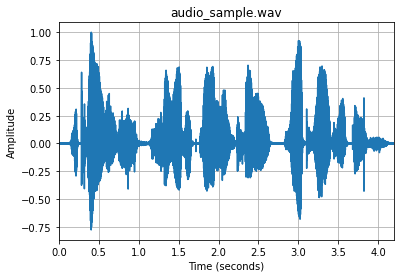
\includegraphics[width=0.5\textwidth]{img/1_sample_signal}
  \caption{Representación de amplitud normalizada frente a tiempo del audio de ejemplo.}
  \label{fig:2_sample_audio}
\end{figure}

\section{Representación de etiquetas de actividad de voz}

\textbf{Pregunta 3}. \textit{¿Qué valores tienen las etiquetas? ¿Qué significan dichos valores? ¿Por qué se representa $\text{voice\_labels}\ast 2-1$?}

\textit{Respuesta}. Las etiquetas tienen valores en $\{0,1\}$, donde $0$ significa silencio y $1$ presencia de voz. A la hora de representarlas se realiza una transformación lineal $0\mapsto -1$ y $1\mapsto 1$ para que encajen los valores de las etiquetas con los valores de amplitud de la señal normalizada en la gráfica, y así poder visualizarlas en la misma escala. Esta transformación corresponde a la fórmula $x\mapsto 2x-1$, de forma que ahora el $-1$ significa silencio y el $1$ sigue siendo presencia de voz.

\textbf{Pregunta 4.} \textit{Represente la señal de voz junto con las etiquetas para ambos etiquetados. ¿Qué diferencias se observan? ¿A qué se puede deber?}

\textit{Respuesta}. La representación de la señal de audio de ejemplo con los dos etiquetados distintos puede observar en la Figura \ref{fig:4}.

\begin{figure}[h!]
     \centering
     \begin{subfigure}[b]{0.45\textwidth}
         \centering
         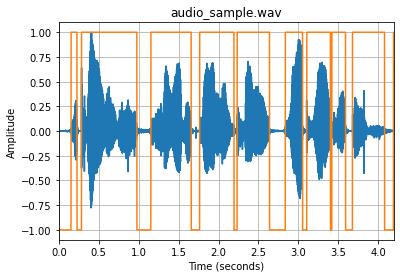
\includegraphics[width=\textwidth]{img/1_sample_labels}
         \caption{Etiquetado 1}
     \end{subfigure}
     \hfill
     \begin{subfigure}[b]{0.45\textwidth}
         \centering
         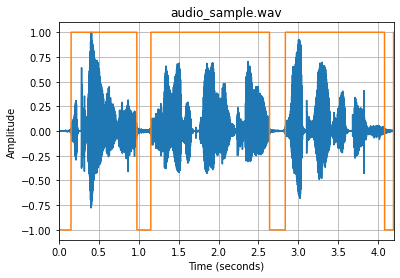
\includegraphics[width=\textwidth]{img/1_sample_labels2}
         \caption{Etiquetado 2}
     \end{subfigure}
        \caption{Representación de la señal de ejemplo junto a dos etiquetados distintos de voz/sliencio.}
        \label{fig:4}
\end{figure}

Vemos que con el primer etiquetado hay más cambios entre voz y silencio que en el segundo. Podríamos decir que el primero es más fino o más específico, mientras que el segundo realiza un etiquetado más grueso. Esto puede deberse a distintos factores, como el diseño del detector de actividad de voz o su propósito. Por ejemplo, el primero podría estar diseñado para reconocer sílabas (recogiendo los silencios entre una y otra), y el segundo para reconocer palabras (solo recogería silencios entre palabras completas). También puede ser simplemente que ambos detectores estén calibrados a distinta resolución, de forma que el segundo solo puede reconocer silencios de una cierta duración mínima (mayor que la del primero) o de una cierta amplitud máxima (menor que la del primero).

\textbf{Pregunta 5.} \textit{¿Qué cantidad de voz/silencio hay en cada etiquetado?}

\textit{Respuesta}. En el primer etiquetado hay más cantidad de silencio que en el segundo. Concretamente, las proporciones de voz/silencio para ambos son:

\begin{table}[h!]
  \centering
  \begin{tabular}{c|cc}
    & Voz & Silencio\\
    \hline
    Etiquetado 1 & 76.26\%&23.74\%\\
    Etiquetado 2 & 84.79\%&15.21\%
  \end{tabular}
\end{table}

\section{Extracción de características}

\textbf{Pregunta 6.} \textit{¿Qué se obtiene de la función \texttt{melspectrogram}? ¿Qué dimensiones de mel\_spec obtienes? ¿Qué significan?}

\textit{Respuesta}. Obtenemos la representación del melespectrograma extraído de la señal, que mide la amplitud de la señal en una malla de frecuencia (en escala Mel) y tiempos discretizados (frames). Concretamente, obtenemos una matriz de tamaño $23\times 420$, donde las filas representan cada una de las 23 divisiones equiespaciadas en las que se ha discretizado la escala Mel, y las columnas cada uno de los instantes de tiempo considerados. Podemos visualizar el melespectrograma obtenido en la Figura \ref{fig:1_mel}.
\begin{figure}[h!]
  \centering
  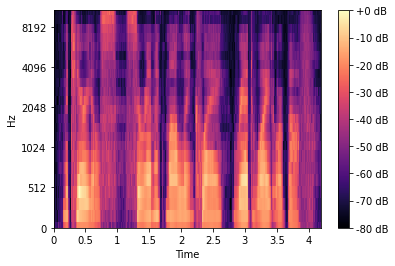
\includegraphics[width=0.5\textwidth]{img/1_mel}
  \caption{Representación del melespectrograma del audio de ejemplo (amplitud en dB).}
  \label{fig:1_mel}
\end{figure}

\textbf{Pregunta 7.} \textit{¿Qué significan los valores de los parámetros win\_length y hop\_length?}

\textit{Respuesta.} El parámetro \textit{win\_length} $=320$ representa el tamaño de ventana que se utiliza para aplicar la transformada de Fourier en cada frame de audio (si es distinto de \textit{n\_fft} se completa con 0s hasta que coincida). Por su parte, el parámetro \textit{hop\_length} $=160$ controla el número de \textit{samples} que hay entre dos frames consecutivos, algo así como el ``salto'' entre ventanas. Notamos que el número de frames (instantes de tiempo en la malla) que obtenemos al final se calcula a partir de este parámetro como
\[
\frac{67072 \text{ samples}}{160 \text{ samples/frames}} = 419.2 \approx 420 \text{ frames}.
\]

\section{Definición del modelo}

\textbf{Pregunta 8}. \textit{¿Qué tamaño tiene la entrada a la capa LSTM? ¿Cuántas unidades (celdas) tiene dicha capa LSTM?}

\textit{Respuesta.} La entrada tiene tamaño \textit{feat\_dim}, que por defecto es 20 (los coeficientes MFCC de los que disponemos para cada frame) y representa el número de características. Hemos configurado la capa LSTM para que tenga 256 celdas.

\textbf{Pregunta 9}. \textit{¿Qué tipo de matriz espera la LSTM? Mirar la documentación y describir brevemente.}

\textit{Respuesta}. La LSTM espera como entrada una matriz de dimensiones (batch, seq, feature), donde \textit{batch} es el tamaño de batch (conjunto de segmentos), \textit{seq} el número de frames de cada segmento, y \textit{feature} el tamaño de la entrada (número de características por cada frame). En nuestro caso, pasaremos tensores de entrada de tamaño $(51, 300, 20)$. Además, aunque nosotros no lo hacemos, se puede pasar también el estado inicial de las celdas y los estados ocultos para cada elemento del batch, que por defecto se inicializan a 0.

\textbf{Pregunta 10.} \textit{Revisar la documentación de torch.nn.LSTM y describir brevemente los argumentos batch\_first, bidirectional y dropout.}

\textit{Respuesta}. El parámetro \textit{batch\_first = True} indica que el tamaño de batch va en la primera dimensión en el tensor de entrada (de lo contrario iría en la segunda). El parámetro \textit{dropout} se utiliza para añadir una capa Dropout de regularización y apagar con cierta probabilidad algunas celdas en tiempo de entrenamiento. Por defecto es \textit{False}, y aunque lo activáramos en nuestro caso concreto no tendría efecto, ya que solo funciona en las capas intermedias, y nunca tras la última capa (nosotros solo estamos usando una capa LSTM). Por último, el parámetro \textit{bidirectional} podría activarse para obtener una red LSTM bidireccional (formada por dos redes que se entrenan sobre la entrada original y sobre la entrada en orden inverso, respectivamente).

\textbf{Pregunta 11}. \textit{En este modelo, estamos utilizando una única neurona a la salida. ¿Hay alguna otra alternativa? ¿Se seguiría utilizando una función sigmoid?}

\textit{Respuesta}. Podríamos emplear dos neuronas a la salida y sustituir la activación sigmoide por una activación softmax, de forma que la salida de la primera neurona representase la probabilidad de voz y la de la segunda la probabilidad de silencio (o viceversa), y ambas sumasen 1. Se elegiría como predicción, obviamente, la de mayor probabilidad.

\textbf{Pregunta 12.} \textit{¿Para qué sirve la función forward definida en la clase Model\_1?}

\textit{Respuesta}. Es la función que indica cómo se realiza el paso hacia delante de los elementos de entrada por la red. Concretamente, recibe como entrada un batch de secuencias de características, al que primero se le aplica la capa LSTM y después la capa fully-connected, formada por una única neurona de salida con activación sigmoide.

\section{Lectura y preparación de los datos para el entrenamiento}

\textbf{Pregunta 13.} \textit{¿Qué tamaño tiene features? ¿Y labels? Una de las dimensiones de la features es 60, correspondiente a los 20 coeficientes MFCC concatenados con las derivadas de primer y segundo orden. ¿Con qué se corresponde la otra dimensión?}

\textit{Respuesta}. Para el audio de entrenamiento \texttt{features\_labs\_1.mat}, \textit{features} tiene tamaño $46654\times 60$ y \textit{labels} $46654\times 1$, y representan las características (20 coeficientes MFCC y las derivadas de primer y segundo orden) y las etiquetas (voz/silencio) de cada frame. Por tanto, la primera dimensión indica el frame concreto que se está evaluando, y en este ejemplo hay 46654 frames en total.

\textbf{Pregunta 14}. \textit{¿De qué tamaño son los fragmentos que se están leyendo? ¿Para qué sirve rand\_idx?}

\textit{Respuesta}. Los fragmentos que se leen son de tamaño \textit{length\_segments}, que hemos fijado en el código a 300 frames. Por su parte, la variable \textit{rand\_idx} es un diccionario que va guardando el frame inicial de cada fragmento procesado (que es aleatorio salvo que la longitud de la señal sea menor de 300, en cuyo caso usamos la señal completa), para poder obtener después las etiquetas correspondientes.

\section{Entrenamiento del modelo}

\textbf{Pregunta 15.} \textit{¿Qué función de coste se está optimizando? Describir brevemente con ayuda de la documentación.}

\textit{Respuesta.} Estamos optimizando la función de coste \textit{BCELoss}. Se trata simplemente del \textit{binary cross-entropy} ó \textit{log-loss} entre etiquetas y predicciones, es decir,
\[
l(y, \hat y) = -\left[ y\log \hat y + (1-y)\log (1-\hat y)\right].
\]
Por defecto se devuelve para cada \textit{batch} la media de las pérdidas individuales entre las etiquetas $y_n$ y las correspondientes predicciones $\hat y_n$.

\textbf{Pregunta 16.} \textit{¿Qué optimizador se ha definido?}

\textit{Respuesta.} Hemos definido un optimizador Adam con tasa de aprendizaje igual a $10^{-3}$. Se trata de un método de descenso por gradiente estocástico que actúa sobre los \textit{batches} de datos, basado en una estimación adaptable de los momentos de primer y segundo orden.

\textbf{Pregunta 17.} \textit{¿Para qué se utiliza batch\_size? Describir brevemente la creación de los batches.}

\textit{Respuesta.} El parámetro \textit{batch\_size} controla el tamaño de cada \textit{batch}, que es el conjunto de secuencias de características que le pasamos al modelo cada vez en el \textit{forward pass}. Para crear estos batches, cogemos secuencias aleatorias de 300 frames (cada uno con 20 características) de los distintos ficheros de entrenamiento, hasta completar el tamaño de batch. De esta forma, en cada época se pasan al modelo distintos batches, y al final de cada una se ha cogido un segmento potencialmente distinto de cada fichero. En nuestro caso hemos fijado el tamaño de batch a 51, de forma que con 10 batches conseguimos recorrer todos los ficheros sin que sobre ninguno.

Para materializar la creación de batches se concatenan los segmentos aleatorios que devuelve la función \texttt{get\_fea} por cada uno de los 51 ficheros asociados a ese batch (concatenación vertical usando \texttt{np.vstack}), y se obtienen las etiquetas correspondientes con \texttt{get\_labels}, que también se concatenan. Después se barajan los datos para añadir aleatoriedad.

\textbf{Pregunta 18.} \textit{¿Qué línea de código realiza el forward pass? ¿Qué línea de código realiza el backward pass?}

\textit{Respuesta.} El \textit{forward pass} se realiza para cada batch en la línea
\begin{minted}{python}
outputs = model(train_batch)
\end{minted}

El \textit{backward pass} por su parte consiste en calcular los gradientes de la pérdida mediante \textit{backpropagation}. Se realiza en:
\begin{minted}{python}
loss.backward()
\end{minted}

Tras esto se realiza un paso del optimizador para actualizar los pesos con los gradientes calculados mediante
\begin{minted}{python}
optimizer.step()
\end{minted}

\textbf{Pregunta 19.} \textit{Añada al código el cálculo de la precisión o accuracy, de tal manera que se muestre por pantalla dicho valor en cada iteración (similar a lo que ocurre con el valor del coste loss). Copiar el código en el informe y describir brevemente.}

\textit{Respuesta}. Concatenamos las etiquetas \textit{ground truth} de todos los frames utilizados en todos los batches de una época (es decir, un total de $10\cdot 51 \cdot 300$), y también las correspondientes etiquetas predichas por el modelo. Para las predicciones es necesario establecer un umbral, pues el modelo solo devuelve la probabilidad de voz. Fijamos este umbral a $0.5$, es decir, diremos que en un frame hay voz si el modelo dice que es más probable que haya voz a que haya silencio. Finalmente calculamos el \textit{accuracy} de la época como la proporción de aciertos.

\begin{minted}{python}
y_pred, y_true = [], []
for ii, segment_set in enumerate(segment_sets):
    ...
    preds = outputs.cpu().detach().numpy().flatten()  # gpu -> cpu
    y_pred.extend([1 if p >= 0.5 else 0 for p in preds])
    y_true.extend(labs_batch.cpu().numpy().flatten())  # gpu -> cpu
y_pred = np.array(y_pred, dtype=np.float32)
y_true = np.array(y_true, dtype=np.float32)
acc = np.mean(y_true == y_pred)
\end{minted}

\textbf{Pregunta 20.} \textit{¿Cuántas iteraciones del algoritmo ha realizado? ¿Qué observa en la evolución de la función de coste? ¿Qué valor de coste y accuracy obtiene? ¿Cómo se puede mejorar?}

\textit{Respuesta.} En total se han realizado 4 iteraciones (épocas) del algoritmo. Podemos ver en la Figura \ref{fig:learning} la evolución del \textit{accuracy} y de la función de coste\footnote{Se ha modificado ligeramente el cálculo de la pérdida para que refleje la pérdida media por cada época, mostrando \texttt{cache\_loss/len(segment\_sets)} al final de cada una.} por cada época.

\begin{figure}[h!]
  \centering
  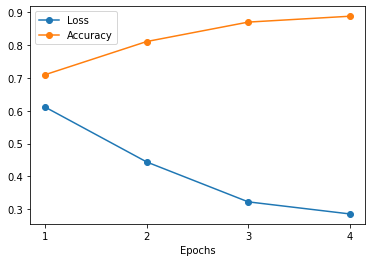
\includegraphics[width=0.5\textwidth]{img/learning_curves}
  \caption{Evolución del coste y la precisión durante el entrenamiento del modelo.}
  \label{fig:learning}
\end{figure}

Como vemos, la función de coste va disminuyendo conforme aumentamos las épocas de entrenamiento, aunque al principio el descenso es más pronunciado y después se suaviza, llegando a un valor de 0.2856 tras la cuarta época. Por su parte, el \textit{accuracy} va creciendo conforme pasan las épocas, también de forma más pronunciada al principio, alcanzando un valor de 88.8\% tras la cuarta época.

En principio podríamos mejorar estos valores (disminuir el coste y aumentar el \textit{accuracy}) entrenando durante más épocas, ya que parece que aún no han llegado al punto de saturación de aprendizaje en el cual se estabilizan. Sin embargo, habría que tener cuidado de no entrenar demasiadas épocas y caer en \textit{overfitting}, o de lo contrario estas mejoras no se verían reflejadas en las predicciones sobre señales que no han sido vistas antes por el modelo.

\section{Evaluación del modelo}

\textbf{Pregunta 21.} \textit{Incluya en el informe de la práctica el código que ha utilizado para evaluar el fichero de audio \texttt{audio\_sample\_test}. ¿Cuál es el accuracy obtenido?}

\textit{Respuesta.} En primer lugar cargamos las características MFCC y las etiquetas del archivo:
\begin{minted}{python}
features_file = 'audio_sample_test.mat'
features = scipy.io.loadmat(features_file)['X'][:, :20]
labels = scipy.io.loadmat(features_file)['Y'].reshape(-1)
\end{minted}

Después, definimos una función para obtener las etiquetas predichas para toda la señal completa (consideramos un solo batch con todos los segmentos, ya que la señal es relativamente pequeña y el paso hacia delante es casi instantáneo):
\begin{minted}{python}
def get_predictions(features):
    model.eval()
    with torch.no_grad():
        batch = features[np.newaxis, :, :]
        batch = torch.tensor(batch.astype("float32")).to(
          torch.device("cuda"))
        preds = model(batch)  # input shape is (1, 57777, 20)
    return preds.cpu().numpy()[0]  # output shape is (57777, 1)
\end{minted}

Finalmente calculamos el \textit{accuracy} como la proporción de aciertos:
\begin{minted}{python}
probs = get_predictions(features)
pred_labels = np.array([1 if p >= 0.5 else 0 for p in probs])
acc = np.mean(labels == pred_labels)
\end{minted}

El \textit{accuracy} obtenido es de $90.9\%$.

\textbf{Pregunta 22.} \textit{Represente 10 segundos de dicho audio, así como sus etiquetas de ground\_truth y las obtenidas con su modelo. Incluya dicha gráfica en el informe y comente brevemente el resultado. Visualmente, ¿es bueno el modelo?}

\textit{Respuesta.} Elegimos representar el audio desde el segundo 10 hasta el 20, usando para ello la función \texttt{plot\_signal}. Además, representamos también las etiquetas de voz/silencio, tanto las de \textit{ground\_trurh} como las predichas por el modelo, y el resultado se puede ver en la Figura \ref{fig:labels}.

\begin{figure}[h!]
     \centering
     \begin{subfigure}[b]{0.49\textwidth}
         \centering
         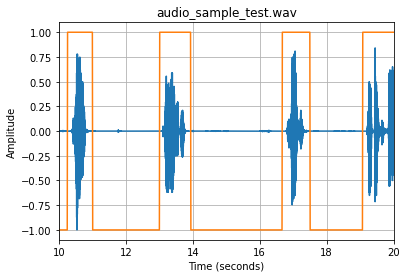
\includegraphics[width=\textwidth]{img/eval_gt}
         \caption{Ground Truth}
     \end{subfigure}
     \hfill
     \begin{subfigure}[b]{0.49\textwidth}
         \centering
         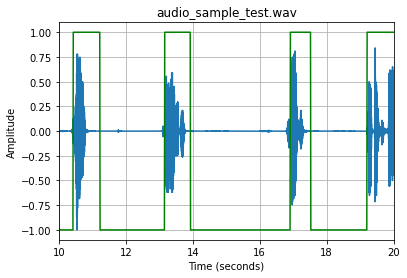
\includegraphics[width=\textwidth]{img/eval_preds}
         \caption{Predicciones}
     \end{subfigure}
        \caption{Representación de la señal de test junto a los etiquetados de \textit{ground\_truth} y los predichos por el modelo.}
        \label{fig:labels}
\end{figure}

Notamos que es necesario cuadrar los tamaños en la representación teniendo en cuenta que en el fichero de características tenemos una muestra (y por tanto una etiqueta) cada 10ms. Así, los puntos sobre los que pintamos las 1000 etiquetas en la gráfica correspondientes a 10s de audio vienen dados por:
\begin{minted}{python}
labels_range = np.linspace(10, 20, num=10/0.01)
\end{minted}

Vemos que las predicciones son buenas, reproduciendo con éxito las etiquetas de voz/silencio de las que disponemos. Visualmente se aprecia como las predicciones se ajustan mejor a los cambios de silencio a voz (aunque en ocasiones quizás apuran demasiado), mientras que el ajuste de los cambios de voz a silencio es peor, al menos en este segmento de audio. En conjunto, podemos decir que el modelo es bastante bueno.

\textbf{Pregunta 23.} \textit{Escuche el audio y comente cualitativamente cómo es de bueno o malo el modelo.}

\textit{Respuesta.} Si escuchamos el audio vemos como entre el segundo 10 y el 20 se escucha una persona diciendo una serie de palabras sueltas con bastante silencio entre ellas, cosa que el modelo captura con éxito. Además, se escucha un pequeño ruido de fondo que el modelo acierta en clasificar como silencio, pues no forma parte de la voz. Sin embargo, aunque nuestro modelo es bueno y reproduce (casi) fielmente los segmentos de silencio y voz del audio original, no puede decirse que el problema sea extremadamente difícil (dentro de lo que podría ser), ya que hay una única voz cuyo sonido es alto, y los silencios son en general largos y sin demasiado ruido de fondo.

Parece que el audio es un único lado de una conversación telefónica, y para este tipo de señales (con las características descritas arriba) nuestro modelo sí parece ser bastante bueno.

\end{document}
